\documentclass[11pt]{article}
\usepackage[margin=0.85in]{geometry}
\usepackage{amsmath,amssymb,graphicx,booktabs,float}
\usepackage[labelfont=bf,font=small]{caption}
\usepackage{hyperref}
\hypersetup{hidelinks}
\setlength{\parindent}{0pt}
\setlength{\parskip}{5pt}
\newcommand{\dt}{\Delta t}
\newcommand{\vect}[1]{\boldsymbol{#1}}
\begin{document}
\begin{center}
{\Large AE 370 Group Project 1}\\[4pt]
{\large Numerical study of a perturbed Earth orbit}\\[5pt]
Jiho Seo, Pranshu Bhardwaj, Adi Jha, Dmitry Moryakov\\
Fall 2026
\end{center}

\section{Premise and equations}\label{sec:premise}
Satellites orbiting Earth are affected by atmospheric drag, Earth's nonspherical gravitational field, and the Moon's gravity. These effects can change a satellite's trajectory and require corrective maneuvers to maintain its orbit. We numerically study these changes and estimate the required velocity corrections.

We address the following questions with matched simulations at two altitudes:
\begin{enumerate}
\setlength{\itemsep}{0pt}
\setlength{\parskip}{0pt}
\item How does atmospheric drag affect the satellite's orbital trajectory over time?
\item How does Earth's gravitational field, including the $J_2$ perturbation, affect the satellite's orbital trajectory?
\item How does the Moon's gravitational influence change the satellite's trajectory, and how does it compare with drag and $J_2$ at different altitudes?
\item How do the numerical method and time step affect the predicted trajectory, particularly when lunar gravity is included?
\item How much additional corrective thrust is required to maintain the desired orbit when the Moon's gravity is included?
\end{enumerate}


The goal of this project is to understand how atmospheric drag, Earth's gravitational field, and the Moon's gravity can change the satellite motion at different altitudes. In addition to that, we need to see how these impacts affect the correction needed in order to keep the orbit intact.

In order to understand these problems, we consider the position and velocity of the satellite in an initial value problem (IVP). The entire system is nonlinear and time-dependent as the gravity force is dependent on the position, the atmosphere resistance force is dependent on the altitude and the velocity and the position of the moon is dependent on the time. Because of the lack of a closed form solution for the entire system, we use numerical solution to find the motion of the satellite.

Let $\vect r=(x,y)^T$, $\vect v=(v_x,v_y)^T$, $r=|\vect r|$, and $h=r-R_E$. In an Earth-centered inertial frame, the state is
\begin{equation}
\vect u=(x,y,v_x,v_y)^T,\qquad
\dot{\vect u}=f(t,\vect u)=
\begin{bmatrix}\vect v\\\vect a_g+\vect a_d+\vect a_{J_2}+\vect a_M\end{bmatrix}.
\label{eq:ode}
\end{equation}
The orbit is equatorial, with $z=0$. Central gravity and the equatorial $J_2$ correction are
\begin{equation}
\vect a_g=-\frac{\mu_E}{r^3}\vect r,\qquad
\vect a_{J_2}=-\frac{3J_2\mu_E R_E^2}{2r^5}\vect r.
\label{eq:gravity}
\end{equation}
We assume a stationary atmosphere, so its relative velocity is $\vect v$:
\begin{equation}
\rho(h)=\rho_0 e^{-(h-h_0)/H},\qquad
\vect a_d=-\frac{C_D A\rho(h)}{2m}|\vect v|\vect v.
\label{eq:drag}
\end{equation}
The prescribed lunar orbit and third-body acceleration are
\begin{equation}
\vect r_M(t)=D\begin{bmatrix}\cos(\omega_M t+\phi_0)\\\sin(\omega_M t+\phi_0)\end{bmatrix},
\qquad \omega_M=\frac{2\pi}{T_M},
\label{eq:moon-orbit}
\end{equation}
\begin{equation}
\vect a_M=\mu_M\left[
\frac{\vect r_M-\vect r}{|\vect r_M-\vect r|^3}
-\frac{\vect r_M}{D^3}\right].
\label{eq:moon}
\end{equation}
The second lunar term subtracts the Moon's acceleration of Earth's center. Omitting it would give the wrong Earth-centered equations. The lunar orbit in Eq.~\eqref{eq:moon-orbit} is idealized: it is circular, it starts at phase $\phi_0=0$ (Section~\ref{sec:maintenance} also tests other phases), and it lies in the satellite's equatorial plane. The real lunar orbit has an eccentricity of about $0.055$ and is inclined about $5.1^\circ$ to the ecliptic, so its inclination to Earth's equator varies between about $18.3^\circ$ and $28.6^\circ$ over an 18.6-year cycle~\cite{moonfacts}. A coplanar Moon cannot exert out-of-plane forces on the satellite, so this assumption also removes any lunar change of the orbital plane. We also neglect the Sun, atmospheric rotation, and changes in satellite mass. Maneuvers are modeled as velocity jumps between ODE integration intervals, as described in Section~\ref{sec:maintenance}.

\section{Parameters and numerical method}\label{sec:method}
All calculations use meters, seconds, and kilograms. Table~\ref{tab:params} lists fixed model inputs, not fitted measurements. The Earth constants $\mu_E$ and $R_E$ are the WGS~84 values~\cite{wgs84}, $J_2$ is the standard value in~\cite{vallado}, $\mu_M$ is the JPL DE430 value~\cite{de430}, and $D$ and $T_M$ are mean values from~\cite{moonfacts}. The density law is a simplified assumption rather than a detailed atmosphere model: $\rho_0$ and $H$ are rounded values of the same order as tabulated exponential-atmosphere values near $400$~km~\cite{vallado}. The satellite mass, area, and drag coefficient are chosen representative values.
\begin{table}[H]
\centering
\caption{Model parameters.}
\label{tab:params}
\begin{tabular}{ll@{\qquad}ll}
\toprule
Parameter & Value & Parameter & Value\\
\midrule
$\mu_E$ & $3.986004418\times10^{14}$ m$^3$/s$^2$ & $R_E$ & $6.378137\times10^6$ m\\
$J_2$ & $1.08263\times10^{-3}$ & $\mu_M$ & $4.9028\times10^{12}$ m$^3$/s$^2$\\
$D$ & $3.84400\times10^8$ m & $T_M$ & $27.32$ days\\
$m$ & $100$ kg & $A$, $C_D$ & $1$ m$^2$, $2.2$\\
$\rho_0$ & $4\times10^{-12}$ kg/m$^3$ & $h_0$, $H$ & $400$ km, $60$ km\\
\bottomrule
\end{tabular}
\end{table}
We use initial altitudes of $300$ km (low) and $35{,}786$ km (high). Each uncontrolled comparison starts with $\vect u_0=(r_0,0,0,\sqrt{\mu_E/r_0})^T$, where $r_0=R_E+h_{\rm initial}$. This is circular for central gravity alone. It is deliberately the same initial state in every physical model, so it need not be circular after $J_2$ is added.

From Lecture 10~\cite{lec10}, integrate the ODE across a step:
\[
\vect u(t_{k+1})-\vect u(t_k)=\int_{t_k}^{t_{k+1}} f(t,\vect u(t))\,dt.
\]
Approximating this integral with staged slopes gives the classical RK4 method:
\begin{align}
 k_1&=f(t_k,\vect u_k),&
 k_2&=f(t_k+\dt/2,\vect u_k+\dt k_1/2),\notag\\
 k_3&=f(t_k+\dt/2,\vect u_k+\dt k_2/2),&
 k_4&=f(t_k+\dt,\vect u_k+\dt k_3),\notag\\
 \vect u_{k+1}&=\vect u_k+\frac{\dt}{6}(k_1+2k_2+2k_3+k_4).\label{eq:rk4}
\end{align}
Each step evaluates these four slopes in order and then updates the state. The time-dependent Moon position is recomputed at each stage time. The integrator is written from scratch, with no outside ODE solver.

We decided to use RK4 as our main numerical method because it is a good balance between accuracy, stability, and computational costs. RK4 is a fourth order method, and Heun is a second order method, so RK4 has less errors for the same time step. Although RK4 has four function evaluations per step compared with two for Heun, its better accuracy makes the additional costs worthwhile. RK4 has a more suitable stability region for oscillatory problems, and Heun can introduce numerical growth for imaginary eigenvalues. We need a method that can accurately capture differences over several days. Therefore, we used RK4 for our main simulations and Heun for comparison.

For comparison, Heun uses $k_1=f(t_k,\vect u_k)$ and a forward Euler prediction $\vect u^*=\vect u_k+\dt k_1$, followed by
\begin{equation}
\vect u_{k+1}=\vect u_k+\frac{\dt}{2}[k_1+f(t_k+\dt,\vect u^*)].
\label{eq:heun}
\end{equation}
It costs two evaluations per step, compared with four for RK4. Taylor expansion gives
$f(t+\dt,u+\dt f)=f+\dt(f_t+f_u f)+O(\dt^2)$.
Thus Heun matches $u(t+\dt)=u+\dt f+\dt^2(f_t+f_u f)/2+O(\dt^3)$: its one-step error is $O(\dt^3)$ and global order is two for a smooth problem over a fixed interval. RK4 has one-step error $O(\dt^5)$ and global order four, as covered in Lecture 10~\cite{lec10}.

Following Lecture 11~\cite{lec11}, truncation error is the residual after substituting the exact solution, divided by $\dt$. For RK4 this is $O(\dt^4)$, rather than the undivided $O(\dt^5)$ step error. The numerical checks below test the expected global orders on the nonlinear orbital equations.

\newpage
\section{Stability and independent validation}\label{sec:stability}
For the lecture test equation $\dot u=\lambda u$, let $w=\dt\lambda$. Substitution into RK4 gives successive slopes proportional to
\[
\lambda u_k,\quad \lambda u_k(1+w/2),\quad
\lambda u_k(1+w/2+w^2/4),\quad
\lambda u_k(1+w+w^2/2+w^3/4).
\]
Collecting terms gives $u_{k+1}=R(w)u_k$, where
\begin{equation}
R_{\rm RK4}(w)=1+w+\frac{w^2}{2}+\frac{w^3}{6}+\frac{w^4}{24},
\quad R_{\rm Heun}(w)=1+w+\frac{w^2}{2}.
\label{eq:stability}
\end{equation}
RK4 matches $e^w$ through degree four. Its test-equation truncation error is
$\tau_k=\lambda^5u(t_k)\dt^4/120+O(\dt^5)$. This verifies the order on the linear test problem; it alone is not a proof for every nonlinear ODE.

Absolute stability requires $|R(w)|<1$ for decay. On the imaginary axis, writing $w=iq$ gives $|R_{\rm RK4}(iq)|^2=1-q^6/72+q^8/576$. Thus RK4 has no amplification for $|q|\le\sqrt8$. Heun instead gives $1+q^4/4>1$ for nonzero $q$, which can cause growth in oscillatory calculations. Stability does not guarantee small phase or position error.

\begin{figure}[H]
\centering
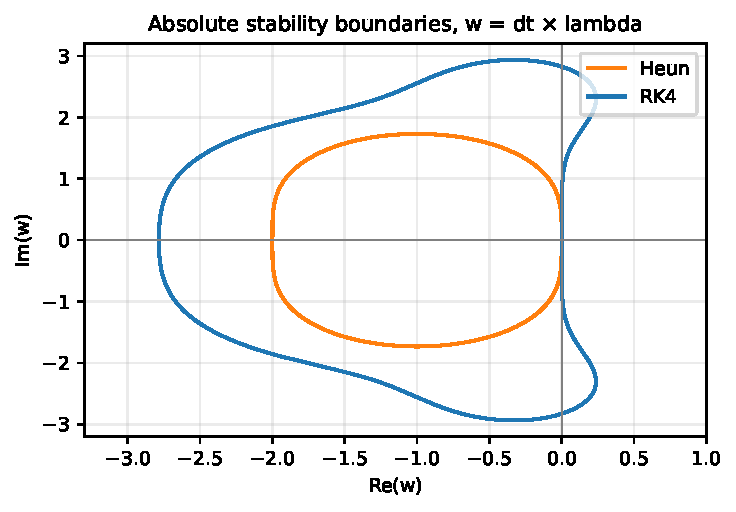
\includegraphics[width=.55\textwidth]{figures/stability.pdf}
\caption{Absolute stability boundaries $|R(w)|=1$ of Eq.~\eqref{eq:stability} for Heun and RK4 in the complex $w=\dt\lambda$ plane.}
\label{fig:stability}
\end{figure}
The curves in Figure~\ref{fig:stability} bound the regions containing small negative real $w$. Our orbit is nonlinear and time dependent, so a fixed scalar test does not establish its full stability. We do not claim stiffness simply because the Moon and satellite have different periods. RK4 is a practical explicit choice, with reliability checked by refinement.

For independent validation, remove drag, $J_2$, and the Moon. At $300$ km the circular solution is
\begin{equation}
\vect r(t)=r_0(\cos nt,\sin nt)^T,\qquad
n=\sqrt{\mu_E/r_0^3},\qquad P=2\pi/n=5431.18\ \mathrm{s}.
\label{eq:exact}
\end{equation}
We compare over three periods using $E=\max_k|\vect r_k-\vect r(t_k)|$. The known solution checks correctness as well as convergence. We also check the specific energy $\epsilon=|\vect v|^2/2-\mu_E/r$ and specific angular momentum $\ell=xv_y-yv_x$, which must be constant in this special case. At the finest RK4 step, their maximum relative changes are $1.49\times10^{-12}$ and $7.45\times10^{-13}$.

\subsection*{Checks of the perturbation terms}
The circular solution tests only central gravity. Three further checks compare the $J_2$ and drag runs with results derived without the integrator. The lunar term has no comparably simple closed form, so it is checked by the refinement study in Section~\ref{sec:convergence}.

\textit{$J_2$ conservation laws.} In the equatorial plane the $J_2$ force is purely radial and derives from the potential $-\mu_E/r-\mu_E J_2R_E^2/(2r^3)$. The specific angular momentum $\ell$ is therefore still conserved, and so is
\begin{equation}
\epsilon_{J_2}=\frac{|\vect v|^2}{2}-\frac{\mu_E}{r}-\frac{\mu_E J_2R_E^2}{2r^3},
\label{eq:j2energy}
\end{equation}
rather than the central-gravity energy $\epsilon$. Over the seven-day $J_2$-only runs, the maximum relative changes of $\epsilon_{J_2}$ and $\ell$ are $1.28\times10^{-10}$ and $6.41\times10^{-11}$ at low altitude, and $6.29\times10^{-11}$ and $3.14\times10^{-11}$ at high altitude.

\textit{$J_2$ radial excursion.} With $\ell^2=\mu_E r_0$, the radial motion is governed by the effective potential $V(r)=\ell^2/(2r^2)-\mu_E/r-\mu_EJ_2R_E^2/(2r^3)$. Let $\kappa=\tfrac32J_2(R_E/r_0)^2$. Then $V'(r_0)=\kappa\mu_E/r_0^2>0$ and $V''(r_0)=\mu_E/r_0^3+O(J_2)$, so the satellite starts at its maximum radius. The other turning point, where $V(r_0-\Delta r)=V(r_0)$, is approximately
\begin{equation}
\Delta r\approx\frac{2V'(r_0)}{V''(r_0)}=2r_0\kappa=\frac{3J_2R_E^2}{r_0}.
\label{eq:j2drop}
\end{equation}
This gives $19.785$~km at low altitude and $3.134$~km at high altitude. Solving $V(r)=V(r_0)$ exactly by bisection gives $19.7849$~km and $3.1336$~km. The simulated minimum radii agree with these exact values to within $1$~m at low altitude and $10$~m at high altitude, consistent with the small energy drift above.

\textit{Drag decay rate.} For a nearly circular orbit, $\epsilon\approx-\mu_E/(2a)$ and $\dot\epsilon=\vect v\cdot\vect a_d$ with $v^2\approx\mu_E/a$ give
\begin{equation}
\dot a\approx-\rho\sqrt{\mu_E a}\,\frac{C_DA}{m}.
\label{eq:dadt}
\end{equation}
At $300$~km this is $2.08$~km/day, or $14.54$~km over seven days if the density stayed fixed. Letting the density follow the falling altitude, with $\sqrt{\mu_E a}$ held at its initial value, gives $\dot h=-c\,e^{-(h-h_0)/H}$ with $c=\rho_0\sqrt{\mu_E r_0}\,C_DA/m$. This integrates to
\begin{equation}
h(t)=h_0+H\ln\left[e^{(h_{\rm initial}-h_0)/H}-\frac{c\,t}{H}\right],
\label{eq:decay}
\end{equation}
which predicts a seven-day loss of $16.649$~km. The simulated drag-only loss is $16.643$~km.

\newpage
\section{Convergence and choice of time step}\label{sec:convergence}
\begin{figure}[H]
\centering
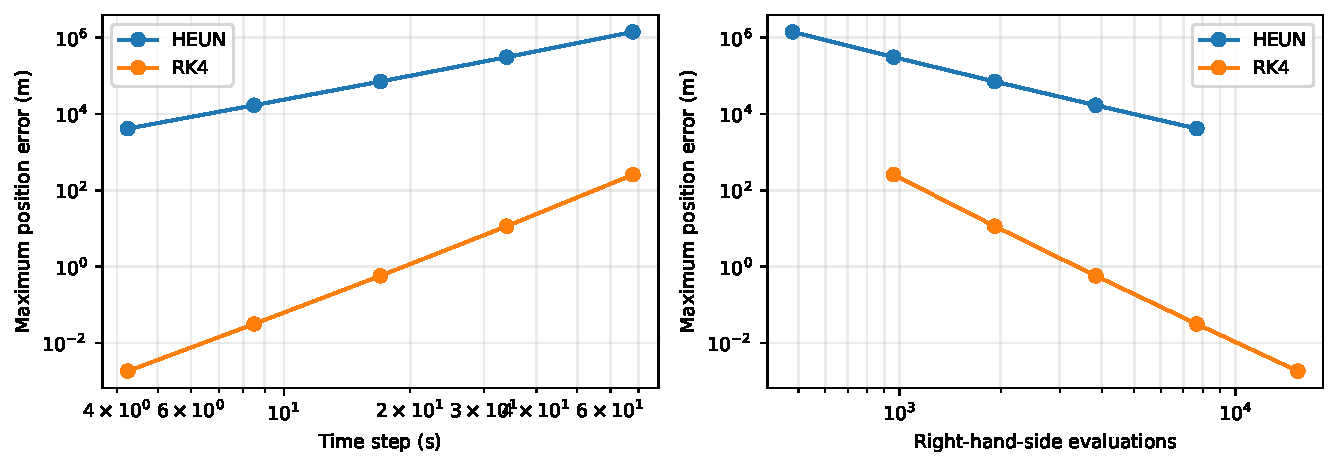
\includegraphics[width=\textwidth]{figures/validation.pdf}
\caption{Exact circular-orbit position errors over three periods. The right panel compares cost by the number of ODE right-hand-side evaluations.}
\label{fig:validation}
\end{figure}

\begin{table}[H]
\centering
\caption{Maximum position error over three periods of the exact circular orbit, Eq.~\eqref{eq:exact}.}
\label{tab:validation}
\begin{tabular}{rrr}
\toprule
$\dt$ (s) & Heun error (m) & RK4 error (m)\\
\midrule
67.8897 & $1.4230\times10^6$ & 257.367\\
33.9449 & $3.1083\times10^5$ & 11.4748\\
16.9724 & $7.1348\times10^4$ & 0.57301\\
8.4862 & $1.7016\times10^4$ & 0.031311\\
4.2431 & $4.1529\times10^3$ & 0.0018218\\
\bottomrule
\end{tabular}
\end{table}
Using $p=\log_2(E(\dt)/E(\dt/2))$ on the last pair gives $p=2.03$ for Heun and $p=4.10$ for RK4. The rates approach the expected two and four. At equal cost of $7680$ evaluations, Heun's error is $4153$ m while RK4's is $0.0313$ m. The measured runtimes of these two short runs were about $0.015$ s and $0.017$ s; such short timings are machine dependent. Evaluation counts are the clearer comparison.

For seven-day results we select $\dt=5$ s at low altitude and $120$ s at high altitude, which is $120{,}960$ and $5{,}040$ steps. On our machine one full-model run takes about $2.4$ s at low altitude and $0.1$ s at high altitude, and the complete script, including every refinement run and the phase sweep of Section~\ref{sec:maintenance}, runs in about one minute. The full model and the baseline are each repeated at half that step. Table~\ref{tab:refinement} gives the maximum coarse--fine differences at common times.
\begin{table}[H]
\centering
\caption{Maximum differences between runs at $\dt$ and $\dt/2$.}
\label{tab:refinement}
\begin{tabular}{lrrr}
\toprule
Orbit & Position, full model & Altitude, full model & Paired lunar displacement\\
 & (m) & (m) & difference (m)\\
\midrule
Low & 1.3773 & 0.004052 & 0.000222\\
High & 0.3185 & 0.009618 & 0.000438\\
\bottomrule
\end{tabular}
\end{table}
The last column compares $(\vect r_{\rm lunar}-\vect r_{\rm base})$ between the two step sizes, where the subscripts denote the full lunar run and the baseline run. It checks the actual difference we interpret as the Moon's effect. These are numerical differences, not rigorous error bounds. Both the individual-run and paired differences are much smaller than the lunar signals reported next. To measure an order on the full equations rather than only on the two-body problem, we also ran the full lunar model at $\dt/4$ ($1.25$ s and $30$ s). The maximum position difference falls from $1.3773$ m ($\dt$ against $\dt/2$) to $0.07084$ m ($\dt/2$ against $\dt/4$) at low altitude, and from $0.3185$ m to $0.01725$ m at high altitude. These give observed orders of $p=4.28$ and $4.21$, consistent with fourth-order convergence on the equations we actually report.

For scale, $n\dt$ is about $0.0058$ in the low orbit and $0.0087$ in the high orbit. This is the relevant size of $w$ because the solution oscillates at the orbital frequency $n$: small perturbations of a circular orbit, written in a frame rotating with the orbit, obey the Clohessy--Wiltshire equations, whose in-plane eigenvalues are $0$ (twice) and $\pm in$~\cite{curtis}. Drag and the Moon change these only slightly, so $w\approx\pm in\dt$ lies near the imaginary axis. These values are small relative to the imaginary-axis limit $\sqrt8$, but the refinement check is still necessary.

\newpage
\section{Physical results over seven days}\label{sec:results}
We compare central gravity alone, central gravity with drag, central gravity with $J_2$, and the baseline containing all three. A fifth run adds the Moon to the baseline. No corrections are applied in this section.
\begin{figure}[H]
\centering
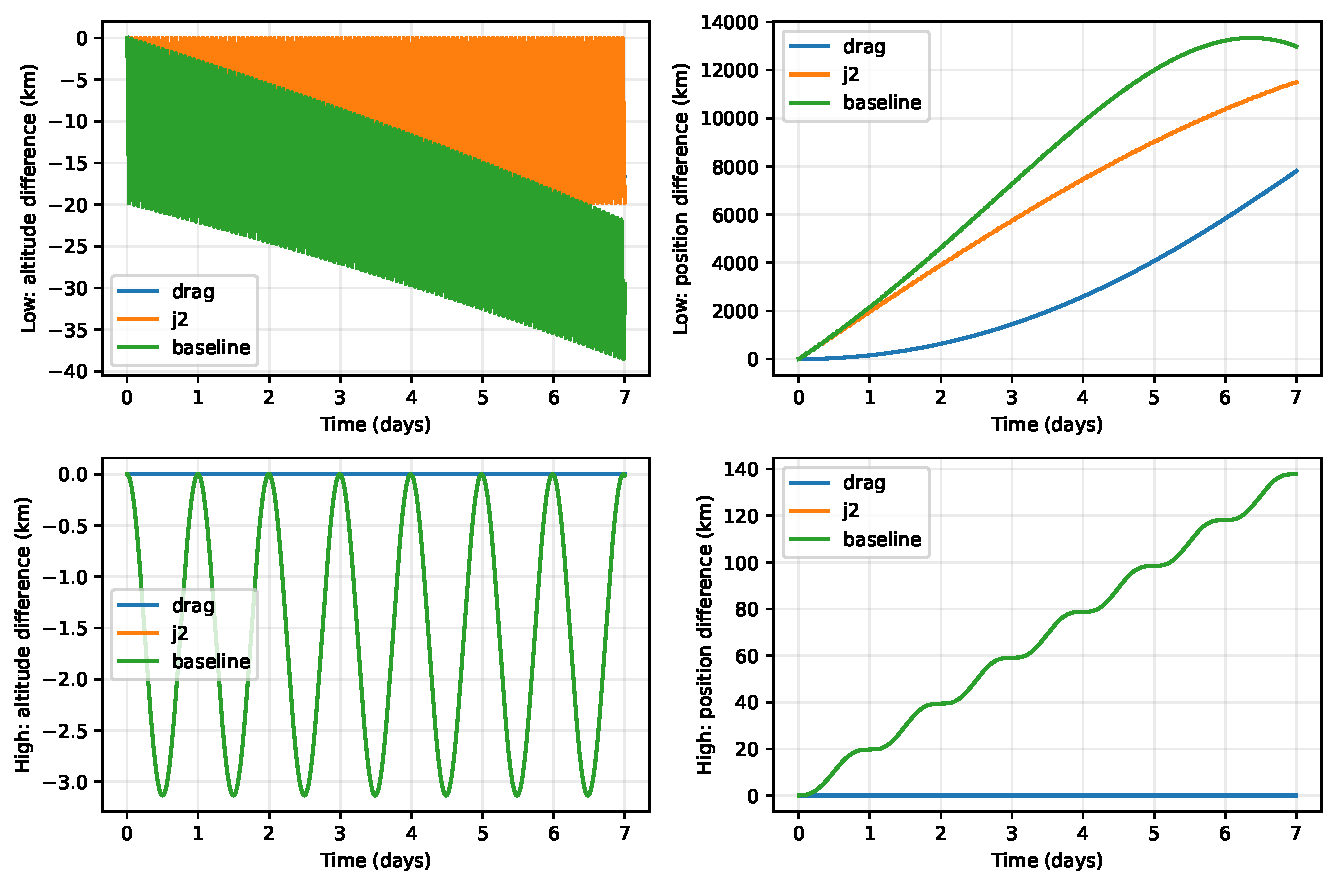
\includegraphics[width=.92\textwidth]{figures/earth_effects.pdf}
\caption{Differences from central gravity alone. The left panels show signed altitude differences; the right panels show position-separation magnitudes. In the low-orbit altitude panel, the slowly falling drag-only curve is hidden behind the $J_2$ and baseline curves, which oscillate rapidly around and below it. In both high-orbit panels the baseline lies exactly on the $J_2$-only curve because drag is negligible there, and the drag-only curve stays at zero.}
\label{fig:earth}
\end{figure}

With drag alone, the low orbit loses $16.643$ km of altitude by day seven, in agreement with the estimate of Eq.~\eqref{eq:decay} (Figure~\ref{fig:earth}). Drag opposes velocity: $\vect v\cdot\vect a_d=-C_D A\rho|\vect v|^3/(2m)\le0$, so it removes orbital energy. The high-orbit density is effectively zero in this exponential model and its drag-only run agrees with central gravity to numerical precision. Extending one density law over this full altitude range is a modeling simplification.

Adding $J_2$ alone gives bounded radial oscillations, reaching $19.785$ km below the initial low altitude and $3.134$ km below the initial high altitude. The initial central-gravity circular speed is too small for a circular orbit in the stronger equatorial gravity field. The size of the excursion matches Eq.~\eqref{eq:j2drop}. These oscillations therefore do not mean that $J_2$ dissipates energy. The central-gravity energy formula is not the full conserved energy after adding $J_2$; the conserved quantity is $\epsilon_{J_2}$ of Eq.~\eqref{eq:j2energy}, which the $J_2$-only runs conserve to about $10^{-10}$. The altered orbital phase also produces large position separations. Our planar model does not describe changes in the orbital plane.

With drag and $J_2$ together, the low altitude reaches a maximum departure of $38.542$ km from its initial value, ending at $270.427$ km. The combined behavior is not a simple sum: lower altitude increases the assumed density and hence the drag. At high altitude the baseline coincides with the $J_2$-only result.

\newpage
\subsection*{Adding lunar gravity}
\begin{figure}[H]
\centering
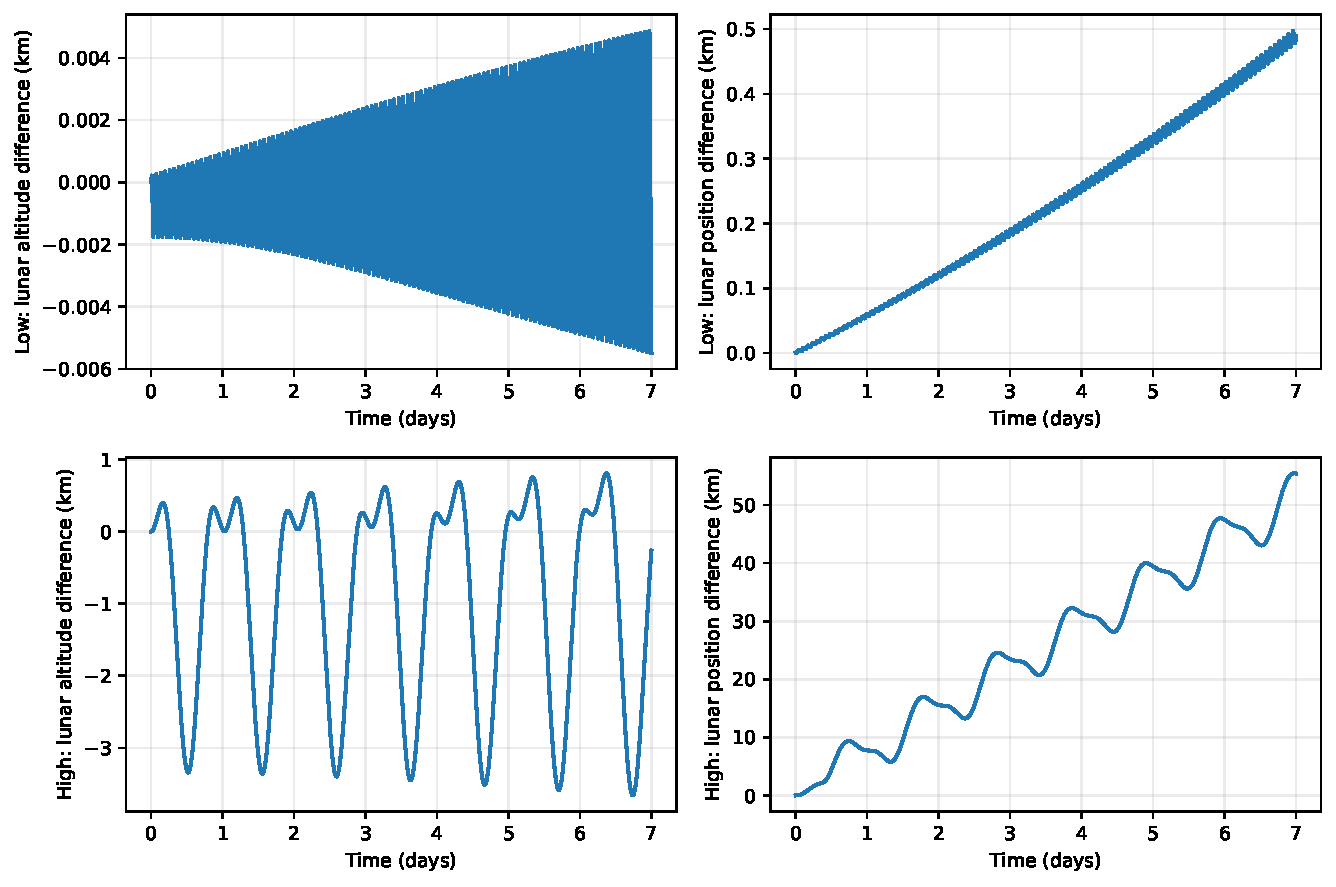
\includegraphics[width=.82\textwidth]{figures/lunar_effect.pdf}
\caption{Full lunar model minus the baseline, with identical initial conditions. Position separation includes phase differences as well as radial differences.}
\label{fig:lunar}
\end{figure}

\begin{table}[H]
\centering
\caption{Seven-day maximum effect of lunar gravity relative to the baseline.}
\label{tab:lunar}
\begin{tabular}{lrr}
\toprule
Seven-day maximum & Low orbit & High orbit\\
\midrule
Lunar position separation (km) & 0.4974 & 55.457\\
Absolute lunar altitude difference (km) & 0.005484 & 3.65995\\
\bottomrule
\end{tabular}
\end{table}
The Moon changes the low-orbit altitude by at most about $5.5$ m relative to the baseline, much less than the drag and $J_2$ effects. Its position difference reaches about $497$ m because small changes in motion can accumulate into phase differences. At high altitude the lunar altitude change is comparable to the $J_2$-only radial excursion, while atmospheric drag is negligible in this model. The lunar position separation reaches about $55.5$ km.

This comparison uses the differential lunar acceleration, not the Moon's direct pull on the satellite alone. Both Earth and satellite respond to the Moon, and that common acceleration is removed. Over larger Earth-centered distances their lunar accelerations differ more strongly. This is consistent with the greater lunar effect in our high orbit.

We also ran Heun on the full lunar model, comparing it with half-step RK4. At low altitude, its maximum position difference falls from $528.5$ km at $5$ s to $98.19$ km at $2.5$ s. At high altitude it falls from $209.9$ km at $120$ s to $49.91$ km at $60$ s. These errors exceed the lunar position signal. A smooth-looking trajectory at these steps would therefore be insufficient evidence of accuracy; method choice matters even when the run does not fail.

The refinement differences in Section~\ref{sec:convergence} are below these signals. However, that only addresses integration error. It does not remove uncertainty caused by the circular Moon orbit, chosen initial phase, or simplified atmosphere. The results apply to this seven-day experiment rather than every satellite or lunar geometry.

\newpage
\section{A simple orbit-maintenance experiment}\label{sec:maintenance}
Every $600$ s we reset velocity while leaving position continuous. Let $r_0$ be the initial radius, $\vect e_r=\vect r/r$, and $\vect e_t=(-y,x)^T/r$. We prescribe
\begin{equation}
v_c(r)=\sqrt{\frac{\mu_E}{r}\left[1+\frac32 J_2\left(\frac{R_E}{r}\right)^2\right]},
\qquad
\vect v^+=v_c(r)\vect e_t-\frac{r-r_0}{3600\ \mathrm{s}}\vect e_r.
\label{eq:control}
\end{equation}
The circular speed follows by setting $v_c^2/r$ equal to the magnitude of central-plus-$J_2$ radial gravity. The radial term points back toward the initial altitude. The checking interval and return time are fixed assumptions; no optimization or advanced control method is used. At each correction,
\begin{equation}
\Delta v_j=|\vect v^+-\vect v^-|,\qquad
\Delta v_{\rm total}=\sum_j\Delta v_j.
\label{eq:dv}
\end{equation}
We use the same rule in the baseline and lunar runs. There are $1008$ corrections over seven days, including the correction at the final time. The rule maintains altitude, not a specified longitude or orbital phase. We use a $3$ km altitude band as a simple success criterion, checking the sampled trajectory between maneuvers as well as at them.
\begin{figure}[H]
\centering
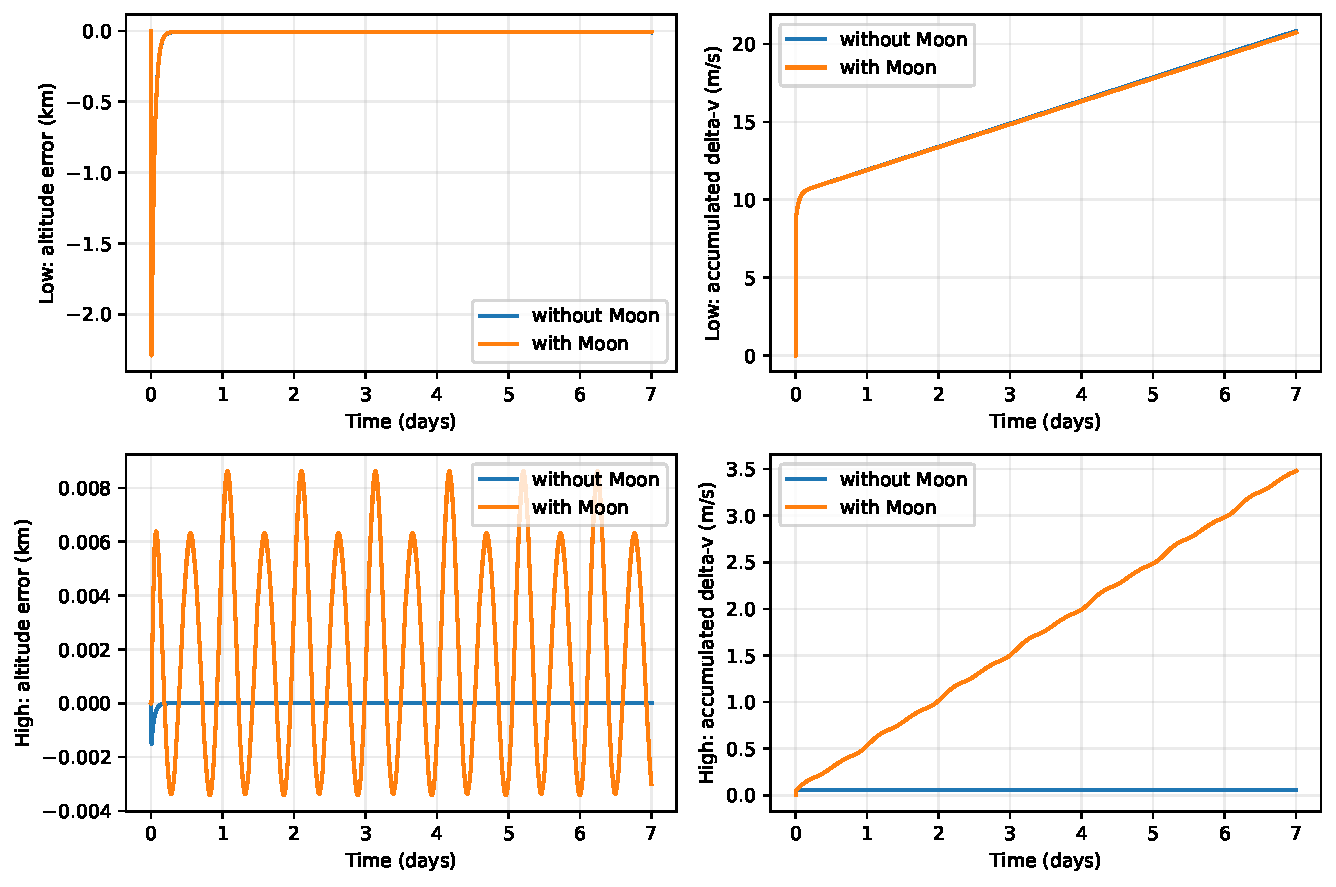
\includegraphics[width=.90\textwidth]{figures/maintenance.pdf}
\caption{Altitude errors and accumulated maneuver magnitudes under the rule of Eq.~\eqref{eq:control}. The nearly overlapping low-orbit curves are expected because its lunar effect is small.}
\label{fig:maintenance}
\end{figure}
\begin{table}[H]
\centering
\caption{Seven-day maintenance cost, Eq.~\eqref{eq:dv}, with initial lunar phase $\phi_0=0$.}
\label{tab:maintenance}
\begin{tabular}{lrr}
\toprule
Quantity & Low orbit & High orbit\\
\midrule
Baseline total $\Delta v$ (m/s) & 20.8366 & 0.05776\\
Lunar total $\Delta v$ (m/s) & 20.7389 & 3.48176\\
Lunar minus baseline $\Delta v$ (m/s) & $-0.09760$ & $+3.42400$\\
Maximum lunar-run altitude error (km) & 2.29046 & 0.008638\\
\bottomrule
\end{tabular}
\end{table}

The control rule shapes these numbers. Without control, the Moon makes the high-orbit radius oscillate by up to about $3.7$ km, roughly once per day (Figure~\ref{fig:lunar}). The rule returns $r$ to $r_0$ within about an hour and resets the speed every $600$ s, so it suppresses this oscillation to under $9$ m (Figure~\ref{fig:maintenance}). It does so by repeatedly cancelling a periodic, largely self-reversing motion instead of letting it average out. Much of the $+3.42$ m/s is therefore the cost of holding a fixed radius tightly under this rule, not a cost the Moon imposes on every maintenance strategy. We did not test a looser rule.

To check sensitivity to the lunar geometry, we repeated the controlled lunar run for eight initial phases $\phi_0$ in Eq.~\eqref{eq:moon-orbit} (Table~\ref{tab:phase}). The baseline does not depend on $\phi_0$.
\begin{table}[H]
\centering
\caption{Lunar minus baseline seven-day $\Delta v$ (m/s) for different initial lunar phases.}
\label{tab:phase}
\begin{tabular}{lrrrrrrrr}
\toprule
$\phi_0$ & $0^\circ$ & $45^\circ$ & $90^\circ$ & $135^\circ$ & $180^\circ$ & $225^\circ$ & $270^\circ$ & $315^\circ$\\
\midrule
Low & $-0.0976$ & $-0.0987$ & $-0.0982$ & $-0.0971$ & $-0.0976$ & $-0.0987$ & $-0.0982$ & $-0.0971$\\
High & $3.424$ & $3.463$ & $3.457$ & $3.438$ & $3.451$ & $3.465$ & $3.434$ & $3.396$\\
\bottomrule
\end{tabular}
\end{table}
The low-orbit difference is negative at every phase tested, between $-0.0987$ and $-0.0971$ m/s, so its sign is not an artifact of choosing $\phi_0=0$. Its values nearly repeat every $180^\circ$, as expected because the dominant tidal part of the lunar perturbation is unchanged when the Moon moves to the opposite side of Earth. The high-orbit increase ranges from $3.396$ to $3.465$ m/s; there the satellite is farther from Earth's center, so the non-tidal part is larger and the $180^\circ$ symmetry is weaker. All of these controlled runs stay within the $3$ km altitude band.

\newpage
\section{Answers to the project questions}\label{sec:answers}
The answers below follow the numbering in the premise.
\begin{enumerate}
\item \textbf{Atmospheric drag.} Drag removes orbital energy and lowers the low orbit. With drag alone, its altitude falls by $16.643$ km in seven days, matching the analytic decay estimate of $16.649$ km (Section~\ref{sec:stability}). Drag is negligible at the high altitude under the assumed density law (Section~\ref{sec:results}, Figure~\ref{fig:earth}).

\item \textbf{Earth's gravity and $J_2$.} Central gravity alone maintains the initial circular orbit. Adding $J_2$ strengthens equatorial gravity, changes the orbital phase, and produces radial oscillations because the same initial speed is no longer circular. Maximum altitude departures with $J_2$ alone are $19.785$ km in the low orbit and $3.134$ km in the high orbit, matching the analytic excursion $3J_2R_E^2/r_0$. This is not drag-like energy loss: the $J_2$ energy $\epsilon_{J_2}$ and angular momentum are conserved to about $10^{-10}$ (Sections~\ref{sec:stability} and~\ref{sec:results}, Figure~\ref{fig:earth}).

\item \textbf{Lunar gravity.} Relative to the baseline, the Moon produces maximum position separations of $0.4974$ km and $55.457$ km in the low and high orbits. Maximum altitude differences are $5.484$ m and $3.65995$ km. Thus the lunar radial effect is much smaller than drag and $J_2$ at low altitude, but comparable to the $J_2$ radial excursion at high altitude, where drag is negligible (Section~\ref{sec:results}, Figure~\ref{fig:lunar}).

\item \textbf{Method and time step.} Independent validation gives convergence orders of $2.03$ for Heun and $4.10$ for RK4. With the Moon included, halving Heun's step reduces its maximum position difference from the fine RK4 reference from $528.5$ to $98.19$ km in the low orbit and from $209.9$ to $49.91$ km in the high orbit. The selected RK4 steps give coarse--fine position differences of only $1.3773$ m and $0.3185$ m, and a further halving gives observed orders of $4.28$ and $4.21$ on the full lunar model. Method choice and refinement are therefore necessary to distinguish lunar effects from numerical error (Sections~\ref{sec:convergence} and~\ref{sec:results}).

\item \textbf{Corrective maneuvers.} For the same maintenance rule, adding the Moon changes the seven-day total $\Delta v$ by $-0.09760$ m/s in the low orbit and $+3.42400$ m/s in the high orbit. Over eight initial lunar phases the low-orbit difference stays negative ($-0.0987$ to $-0.0971$ m/s) and the high-orbit increase ranges from $3.396$ to $3.465$ m/s. All controlled lunar runs stay within the selected $3$ km altitude band at sampled times (Section~\ref{sec:maintenance}, Figure~\ref{fig:maintenance}, Table~\ref{tab:phase}). These are impulse costs, not engine forces: force would also require specifying burn durations. Both numbers are specific to our maintenance rule. At high altitude much of the cost comes from the rule cancelling the Moon's periodic radial oscillation, and the negative low-orbit difference is not a general reduction in maintenance cost.
\end{enumerate}

\subsection*{Limits of these answers}
Halving the step changes the signed maneuver-cost differences by $1.15\times10^{-6}$ m/s at low altitude and $1.23\times10^{-5}$ m/s at high altitude, well below the reported changes. These checks address integration error, not physical-model uncertainty. Apart from the maintenance phase sweep, the results use one lunar phase. They also use a prescribed circular Moon orbit in the equatorial plane, one maintenance rule, a simplified atmosphere, and fixed satellite parameters. The planar model cannot describe orbital-plane changes. The impulse totals include adjustment from the initial central-gravity circular orbit to the $J_2$ model and are not optimal station-keeping costs.

\newpage
\section{Reproducibility and contributions}
The submission contains \texttt{simulation.py}, \texttt{results.json}, the figures, this LaTeX source, and the compiled PDF. Running \texttt{python simulation.py} reproduces all calculations and figures in about one minute, including the perturbation-term checks, the $\dt/4$ convergence run, and the phase sweep, which are written to \texttt{results.json}. The integrators, checks, experiments, and plotting are separate functions within one script. Only NumPy and Matplotlib are required. To rebuild the PDF after generating the figures, compile \texttt{report.tex} with LaTeX.


\subsection*{Group Contributions}
% TODO (team): replace each entry with specifics -- which functions in simulation.py,
% which report sections, and which figures each person wrote -- and make it consistent
% with the Generative AI statement below and the course AI policy.

\begin{itemize}
    \item \textbf{Jiho Seo (25\%):} Contributed to creating the problem statement, choosing the numerical methods, implementing the simulations, and analyzing the results.

    \item \textbf{Pranshu Bhardwaj (25\%):} Worked on the math modeling, numerical implementation, convergence testing, and interpreting the simulation results.

    \item \textbf{Adi Jha (25\%):} Participated in defining the project questions, developing the numerical methods, generated figures, and evaluated the accuracy of the results.

    \item \textbf{Dmitry Moryakov (25\%):} Helped implement and validate the simulations, compare numerical methods, analyze the orbital behavior, and helped prepare the technical report.
\end{itemize}


\section*{Generative AI}
% TODO (team): check this against the course AI policy and the contributions above.
OpenAI ChatGPT assisted with interpreting the supplied materials, planning the experiments, implementing and checking the code, producing figures, and drafting and compiling this report. Anthropic Claude assisted with a later revision: adding the perturbation-term checks, the $\dt/4$ convergence run, and the lunar-phase sweep to \texttt{simulation.py}, and revising the report text, captions, equation numbering, and references.
% TODO (team): add the exact lecture titles and instructor for the two course references.
\begin{thebibliography}{9}
\bibitem{lec10} AE 370 lecture notes, Lecture 10, Fall 2026.
\bibitem{lec11} AE 370 lecture notes, Lecture 11, Fall 2026.
\bibitem{vallado} D.~A. Vallado, \emph{Fundamentals of Astrodynamics and Applications}, 4th ed., Microcosm Press, 2013.
\bibitem{curtis} H.~D. Curtis, \emph{Orbital Mechanics for Engineering Students}, 3rd ed., Butterworth-Heinemann, 2014.
\bibitem{wgs84} National Imagery and Mapping Agency, \emph{Department of Defense World Geodetic System 1984}, Technical Report TR8350.2, 3rd ed., 2000.
\bibitem{de430} W.~M. Folkner, J.~G. Williams, D.~H. Boggs, R.~S. Park, and P.~Kuchynka, ``The planetary and lunar ephemerides DE430 and DE431,'' \emph{IPN Progress Report} 42-196, 2014.
\bibitem{moonfacts} D.~R. Williams, ``Moon Fact Sheet,'' NASA Space Science Data Coordinated Archive, \url{https://nssdc.gsfc.nasa.gov/planetary/factsheet/moonfact.html}.
\end{thebibliography}
\end{document}
